\documentclass[pdf]{beamer}

\mode<presentation>{}

%% Preamble
\usetheme{Madrid}
\usecolortheme{seahorse}
\usefonttheme{professionalfonts}

\setbeamertemplate{section in toc}{\inserttocsectionnumber.~\inserttocsection}
\setbeamertemplate{subsection in toc}{%
  \hspace{1.2em}{\color{blue}\rule[0.3ex]{3pt}{3pt}}~\inserttocsubsection\par}
\setbeamertemplate{itemize items}{%
  \color{blue}\rule[0.3ex]{3pt}{3pt}}

\usepackage{minted}

%% Hide syntax errors in minted
\AtBeginEnvironment{minted}{%
  \renewcommand{\fcolorbox}[4][]{#4}}

%% Set minted to remove preceeding space and set font size
\setminted[]{fontsize=\footnotesize,autogobble}

\usepackage{dirtree}
\usepackage{hyperref}

\hypersetup{
  colorlinks=true,
  linkcolor=black,
  urlcolor=cyan
}

\usepackage{graphicx}
\graphicspath{ {images/} }

\usepackage{etoolbox}

%% Remove extra spacing between sections in the table of contents
\makeatletter
\patchcmd{\beamer@sectionintoc}{\vskip1.5em}{\vskip0em}{}{}
\makeatother

\AtBeginSection[]
{
  \begin{frame}{Table of Contents}
    \tableofcontents[currentsection,hideothersubsections]
  \end{frame}
}

\title{Building a Blogging System}
\subtitle{with Haskell and Yesod}
\author{Gavin Whelan}

\begin{document}

%% title frame
\begin{frame}
  \titlepage
\end{frame}

\begin{frame}{About Me}
  IU CS Graduate\\
  Hunger Prevention Manager\\
  \\
  My "site": \href{https://ambientmemory.com}{ambientmemory.com}\\
  GitHub: \href{https://github.com/gavwhela}{@gavwhela}\\
  \\
  CTO Whiteboard Dynamics LLC\\
  Company site: \href{https://whiteboarddynamics.co}{whiteboarddynamics.co}\\
\end{frame}

\begin{frame}{Attributions}
  This presentation uses resources from the Yesod Book.\\
  \url{https://github.com/yesodweb/yesodweb.com-content}\\
  \url{http://www.yesodweb.com/book}\\
  \\
  As well as the yesod-postgres template.\\
  \href{https://github.com/commercialhaskell/stack-templates/blob/master/LICENSE}{MIT License}\\
\end{frame}

%% \begin{frame}{Layout}
%%   \begin{itemize}
%%   \item<1-> Basic background
%%   \item<2-> Set up Codio \& Dive into an exercise
%%   \item<3-> Routing \& Templating intro
%%   \item<4-> Start building on the scaffolding
%%   \item<5-> Sessions
%%   \item<6> Lunch
%%   \end{itemize}
%% \end{frame}
%% 
%% \begin{frame}{Layout}
%%   \begin{itemize}
%%   \item<1-> Lunch
%%   \item<2-> Starting the blog
%%   \item<3-> Database Storage
%%   \item<4-> Authentication and Authorization
%%   \item<5-> Snack
%%   \end{itemize}
%% \end{frame}
%% 
%% \begin{frame}{Layout}
%%   \begin{itemize}
%%   \item<1-> Snack
%%   \item<2-> Esqueleto
%%   \item<2> Finishing up
%%   \end{itemize}
%% \end{frame}

\section{Basic Background}

\subsection{Language Extensions}
\begin{frame}[fragile]{Overloaded Strings}
  \begin{minted}[frame=single]{haskell}
    class IsString a where
        fromString :: String -> a
  \end{minted}
  \pause
  \vspace{1em}
  Without OverloadedStrings
  \begin{minted}[frame=single]{haskell}
    "Literal String" :: String
    "Literal String" :: [Char]
  \end{minted}
  \pause
  \vspace{1em}
  With OverloadedStrings
  \begin{minted}[frame=single]{haskell}
    {-# LANGUAGE OverloadedStrings #-}
    "Literal String" :: IsString a => a
  \end{minted}
\end{frame}

\begin{frame}[fragile]{Type Families}
  \begin{minted}{haskell}
    {-# LANGUAGE TypeFamilies #-}
    import Data.Word (Word8)
    import qualified Data.ByteString as S
    
    class SafeHead a where
        type Content a
        safeHead :: a -> Maybe (Content a)
    
    instance SafeHead [a] where
        type Content [a] = a
        safeHead [] = Nothing
        safeHead (x:_) = Just x
    
    instance SafeHead S.ByteString where
        type Content S.ByteString = Word8
        safeHead bs
            | S.null bs = Nothing
            | otherwise = Just $ S.head bs
  \end{minted}
\end{frame}

\begin{frame}[fragile]{Template Haskell}
  \begin{minted}{haskell}
    {-# LANGUAGE TemplateHaskell #-}
    
    -- | Template Haskell (TH) is Haskell's approach to code
    -- generation. Yesod uses TH to reduce boilerplate. Code from
    -- before a TH splice cannot refer to code within the TH, or what
    -- follows.

    $(templateHaskellFunction arg1 arg2)

    -- | Or at the top level
    templateHaskellFunction arg1 arg2
  \end{minted}
\end{frame}

\begin{frame}[fragile]{QuasiQuotes}
  \begin{minted}{haskell}
    {-# LANGUAGE QuasiQuotes #-}
    
    -- | QuasiQuotes (QQ) allows arbitrary content to be taken inline
    -- in Haskell code and processed, generating Haskell code as TH does.

    -- | The name of the quasi-quoter is given between the opening
    -- bracket and the first pipe. The quasi-quoted region is closed
    -- with |]

    [hamlet|<p>This is quasi-quoted Hamlet.|]
  \end{minted}
\end{frame}

\subsection{Minimal Example}
\begin{frame}[fragile]{Minimal Example}
  \begin{minted}{haskell}
    {-# LANGUAGE OverloadedStrings #-}
    {-# LANGUAGE QuasiQuotes       #-}
    {-# LANGUAGE TemplateHaskell   #-}
    {-# LANGUAGE TypeFamilies      #-}
    import Yesod

    data HelloWorld = HelloWorld

    mkYesod "HelloWorld" [parseRoutes|
    / HomeR GET
    |]

    instance Yesod HelloWorld

    getHomeR :: Handler Html
    getHomeR = defaultLayout [whamlet|Hello World!|]

    main :: IO ()
    main = warp 3000 HelloWorld
  \end{minted}
\end{frame}

\begin{frame}{Minimal Example: Result}
  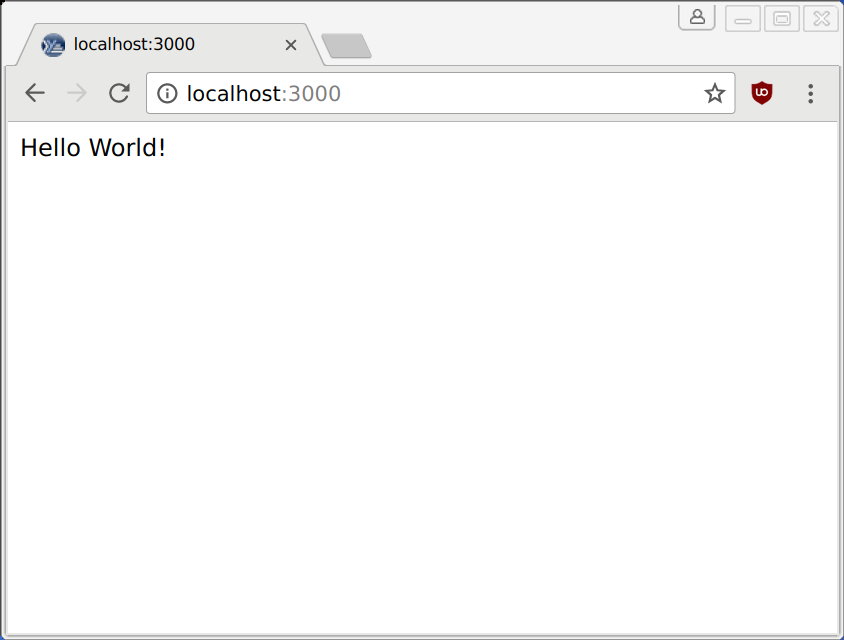
\includegraphics[width=\textwidth,height=0.8\textheight,keepaspectratio]{example}
\end{frame}

%%%%%%%% Maybe put something about setTitle here or something

\section{Set up Codio \& Dive into an exercise}

\subsection{Codio}
\begin{frame}{Setting up Codio}

\end{frame}

\subsection{First Exercise}
\begin{frame}[fragile]{First Exercise}
  \begin{minted}{haskell}
    {-# LANGUAGE OverloadedStrings, QuasiQuotes #-}
    {-# LANGUAGE TemplateHaskell, TypeFamilies  #-}
    import Yesod

    data Links = Links

    mkYesod "Links" [parseRoutes|
    /      HomeR  GET
    /page1 Page1R GET
    /page2 Page2R GET
    |]

    instance Yesod Links

    getHomeR  = defaultLayout [whamlet|<a href=@{Page1R}>Go to page 1!|]
    getPage1R = defaultLayout [whamlet|<a href=@{Page2R}>Go to page 2!|]
    getPage2R = defaultLayout [whamlet|<a href=@{HomeR}>Go home!|]

    main = warp 3000 Links
  \end{minted}
\end{frame}

%% ~25 minutes in I think

\subsection{What did we do?}

\begin{frame}[fragile]{Foundation Datatype}
  Remember these lines?
  \begin{minted}[frame=single]{haskell}
    data Links = Links

    instance Yesod Links
  \end{minted}
  \pause
  
  Links is your foundation datatype, in this example it doesn't
  actually store any data, but it can be a good place to keep settings
  and values requiring initalization before your application starts
  running, such as database connections. Every handler has access to
  data present in the foundation datatype.
\end{frame}

\begin{frame}[fragile]{Yesod Typeclass}
  The Yesod typeclass gives a central place for defining settings for
  the application. Every method has intelligent defaults, so no
  implementation is required, however extensive modification is
  possible.

  \begin{minted}[frame=single]{haskell}
    class RenderRoute site => Yesod site where
        approot :: Approot site
        errorHandler :: ErrorResponse -> Handler TypedContent
        defaultLayout :: Widget -> Handler Html
        isAuthorized :: Route site -> Bool -> Handler AuthResult
        authRoute :: site -> Maybe (Route site)
        makeSessionBackend :: site -> IO (Maybe SessionBackend)
        yesodMiddleware :: ToTypedContent res => Handler res -> Handler res
        defaultMessageWidget :: Html -> HtmlUrl (Route site) -> Widget
  \end{minted}
\end{frame}

\section{Routing \& Templating intro}
\subsection{Routing DSL}
\begin{frame}[fragile]{Routing DSL}
  Declares the routing of paths to handlers or subsites. Specifies
  allowed HTTP methods.

  \begin{minted}[frame=single]{haskell}
    /             HomeR     GET
    /blog         BlogR     GET POST
    /blog/#BlogId BlogPostR GET POST

    /static       StaticR Static getStatic
  \end{minted}
\end{frame}

\begin{frame}[fragile]{Routing DSL}
  Generates a route data type using the resource names.
  %%%%%%% Actually mkYesod fix this
  \begin{minted}[frame=single]{haskell}
    data MyRoute = HomeR
                 | BlogR
                 | BlogPostR BlogId
  \end{minted}
\end{frame}

\subsection{Shakespearean Templating}
\begin{frame}{Shakespearean Templating}
  General purpose templating languages\\
  \\
  \begin{tabular}{ l l }
    Hamlet  & (HTML)\\
    Lucius  & (CSS)\\
    Cassius & (CSS)\\
    Julius  & (JavaScript)\\
  \end{tabular}
\end{frame}

\begin{frame}{Common}
  \#\{...\} Variable interpolation\\
  @\{...\} URL Interpolation\\
  @?\{...\} URL Interpolation w/ query parameters\\
  \textasciicircum\{...\} Template Embedding\\
\end{frame}

\begin{frame}{Hamlet}
  Whitespace based, no closing tags (except same line)\\
  \\
  . as shortcut for class=\\
  \# as shortcut for id=\\
  :...:...: optional attribute\\
  Quotes optional\\
  \$case \$of \\
  \$with \\
  \$doctype \\
  \$forall \\
  \$maybe \$nothing\\
  \$if \$elseif \$else\\
\end{frame}

\begin{frame}[fragile]{Hamlet}
  \begin{minted}{HTML}
    $doctype 5
    <html>
        <head>
            <title>#{pageTitle} - My Site
            <link rel=stylesheet href=@{Stylesheet}>
        <body>
            <h1 .page-title>#{pageTitle}
            <p>Here is a list of your friends:
            $if null friends
                <p>Sorry, I lied, you don't have any friends.
            $else
                <ul>
                    $forall Friend name age <- friends
                        <li>#{name} (#{age} years old)
            <footer>^{copyright}
  \end{minted}
\end{frame}

\begin{frame}{Lucius}
  Mostly a superset of CSS\\
  Nested blocks\\
  Define variables\\
  Mixins\\
\end{frame}

\begin{frame}[fragile]{Lucius}
  \begin{minted}{CSS}
    @textcolor: #494949;                      /* Variable definition */
    body {
        color: #{textcolor};                  /* Variable interpolation */
        font-size: 16px;
    }
    .footer {
        background: url(@{BackgroundImageR}); /* URL interpolation */
        height: 150px;
        text-align: center;
        > .container {                        /* Nested block */
            padding: 45px 0 0 0;
        }
        p {
            margin-top: 45px;
            margin-bottom: 0px;
        }
    }
  \end{minted}
\end{frame}

\begin{frame}[fragile]{Cassius}
  Just Lucius, but whitespace instead of brackets and semicolons.\\
  You don't see this used too much.\\
  \begin{minted}[frame=single]{CSS}
    @textcolor: #494949
    body
        color: #{textcolor}
        font-size: 16px
    .footer
        background-image: url(@{BackgroundImageR})
        height: 150px
        text-align: center
        > .container
            padding: 45px 0 0 0
        p
            margin-top: 45px
            margin-bottom: 0px
  \end{minted}
\end{frame}

\begin{frame}{Julius}
  Just JavaScript with interpolation\\
\end{frame}

\begin{frame}[fragile]{QuasiQuoters}
  \begin{minted}{haskell}
    [hamlet|<h1>My Title|]
    [lucius|h1 { color: green } |]
  \end{minted}
\end{frame}

\begin{frame}{Functions}
  \begin{center}
    \begin{tabular}{ |c|c|c|c| }
      \hline
      Language & QuasiQuoter & External File & Reload\\
      \hline
      Hamlet & hamlet & hamletFile & N/A\\
      \hline
      Cassius & cassius & cassiusFile & cassiusFileReload\\
      \hline
      Lucius & lucius & luciusFile & luciusFileReload\\
      \hline
      Julius & julius & juliusFile & juliusFileReload\\
      \hline
    \end{tabular}
  \end{center}
\end{frame}

\section{Start building on the scaffolding}

\subsection{Widgets}
\begin{frame}{Widgets}
  Yesod's solution to modular and composable web elements. \\
  Each widget has these components:\\
  \begin{itemize}
  \item<1-> The title
  \item<2-> External stylesheets
  \item<2-> External Javascript
  \item<3-> CSS declarations
  \item<3-> Javascript code
  \item<4-> Arbitrary \textless head\textgreater\ content
  \item<4-> Arbitrary \textless body\textgreater\ content
  \end{itemize}
\end{frame}

\begin{frame}[fragile]{Widget Monad}
  Widgets can be composed monadically.
  \begin{minted}[frame=single,escapeinside=??]{haskell}
    myWidget1 = do
      toWidget [hamlet|<h1>My Title|]
      toWidget [lucius|h1 { color: green } |]
    ?\pause?
    myWidget2 = do
      setTitle "My Page Title"
      addScriptRemote "http://www.example.com/script.js"
    ?\pause?
    myWidget = do
      myWidget1
      myWidget2
  \end{minted}
\end{frame}

\subsection{Scaffolding Structure}
\begin{frame}{Site Scaffolding}
  \dirtree{%
    .1 Project/.
    .2 app/\DTcomment{General execution wrappers}.
    .2 config/\DTcomment{Configuration loaded by the application}.
    .2 Handler/\DTcomment{Files containing handlers}.
    .2 Import/.
    .2 Settings/.
    .2 static/.
    .2 templates/.
    .2 Application.hs.
    .2 Foundation.hs.
    .2 Import.hs.
    .2 project.cabal.
    .2 LICENSE.
    .2 Settings.hs.
    .2 stack.yaml.
  }
\end{frame}

%%  \dirtree{%
%%    .1 Project/.
%%    .2 app/.
%%    .3 devel.hs.
%%    .3 DevelMain.hs.
%%    .3 main.hs.
%%    .2 config/.
%%    .3 client\_session\_key.aes.
%%    .3 favicon.ico.
%%    .3 robots.txt.
%%    .3 routes.
%%    .3 settings.yml.
%%    .2 Handler/.
%%    .3 Common.hs.
%%    .3 Home.hs.
%%    .2 Import/.
%%    .3 NoFoundation.hs.
%%    .2 Settings/.
%%    .3 StaticFiles.hs.
%%    .2 static/.
%%    .2 templates/.
%%    .3 default-layout-wrapper.hamlet.
%%    .3 default-layout.hamlet.
%%    .3 default-message-widget.hamlet.
%%    .3 homepage.hamlet.
%%    .2 Application.hs.
%%    .2 Foundation.hs.
%%    .2 Import.hs.
%%    .2 project.cabal.
%%    .2 LICENSE.
%%    .2 Settings.hs.
%%    .2 stack.yaml.
%%  }

\subsection{Sessions}

\begin{frame}{Sessions}
  A session is a way to keep state about an interaction with a
  client. This is generally something that is desired to be minimized,
  but is fairly often unavoidable, such as a shopping cart
  implementation. \\

  Sessions stored on the server are available, but not the default due
  to the additional overhead of doing additional database lookups to
  service requests. \\

  Instead the approach usually used by Yesod is to store the session
  in a cookie on the client. This cookie is encrypted to prevent
  inspection and signed to prevent tampering.
\end{frame}

\begin{frame}[fragile]{Sessions}
  The client session is actually enabled in the default sessionBackend
  implementation, but the scaffolding we are using overrides it to
  change the location of the file that stores the encryption key for
  the cookies. \\

  \begin{minted}[frame=single]{haskell}
    -- Store session data on the client in encrypted cookies,
    -- default session idle timeout is 120 minutes
    makeSessionBackend _ = Just <$> defaultClientSessionBackend
        120    -- timeout in minutes
        "config/client_session_key.aes"
  \end{minted}
\end{frame}

\begin{frame}[fragile]{Sessions}
  Sessions in Yesod are modeled as a basic key value store. \\

  \begin{minted}[frame=single]{haskell}
    type SessionMap = Map Text ByteString
    lookupSession :: MonadHandler m => Text -> m (Maybe Text)
    lookupSessionBS :: MonadHandler m => Text -> m (Maybe ByteString)
    getSession :: MonadHandler m => m SessionMap
    setSession :: MonadHandler m => Text -> Text -> m ()
    setSessionBS :: MonadHandler m => Text -> ByteString -> m ()
    deleteSession :: MonadHandler m => Text -> m ()
    clearSession :: MonadHandler m => m ()
  \end{minted}
\end{frame}

\begin{frame}{Messages}
  One major use of sessions is messages. These solve a common case:
  the user performs a POST request, the web app takes the required
  action, and then wants to simultaneously redirect the user to a new
  page and display a message indicating the result of the
  action. (This is known as Post/Redirect/Get). \\

  Yesod provides a pair of functions to make handling this workflow
  easy: setMessage stores a message in the session, and getMessage
  both reads this message and deletes it from the store to prevent it
  from being displayed again. \\

  The common approach is to check for messages in defaultLayout so
  that the message can be shown to the user immediately, without
  having to add getMessage calls in every handler.
\end{frame}

\begin{frame}[fragile]{Messages}
  This is included in our scaffolding's defaultLayout. \\

  \begin{minted}[frame=single]{haskell}
    defaultLayout widget = do
      master <- getYesod
      mmsg <- getMessage

      pc <- widgetToPageContent $(widgetFile "default-layout")
      withUrlRenderer
        $(hamletFile "templates/default-layout-wrapper.hamlet")
  \end{minted}
  \vspace{0.5em}
  \begin{minted}[frame=single]{HTML}
    <div #wrapper>
      <div .container>
        $maybe msg <- mmsg
          <div #message>#{msg}

      <div .container>
        ^{widget}
  \end{minted}
\end{frame}

\subsection{Before Lunch review}

\section{Lunch}

\section{Starting the Blog}

\section{Authentication and Authorization}
\begin{frame}{Authentication and Authorization}
  
\end{frame}

\subsection{YesodAuth Typeclass}
\begin{frame}[fragile]{YesodAuth Typeclass}
  Minimal complete definition: loginDest, logoutDest,
  (authenticate$|$getAuthId), authPlugins, authHttpManager \\
  \\
  \begin{minted}[frame=single]{haskell}
    class (Yesod site) => YesodAuth site where
        type AuthId site
        authLayout :: Widget -> Handler Html
        loginDest :: site -> Route site
        logoutDest :: site -> Route site
        authenticate :: Creds site -> Handler (AuthenticationResult site)
        getAuthId :: Creds site -> Handler (Maybe (AuthId site))
        authPlugins :: site -> [AuthPlugin site]
        loginHandler :: HandlerT Auth Handler Html
        redirectToReferer :: site -> Bool
        authHttpManager :: site -> Manager
  \end{minted}
\end{frame}

\subsection{isAuthorized}
\begin{frame}[fragile]{isAuthorized}
  \begin{minted}{haskell}
    data AuthResult = Authorized
                    | AuthenticationRequired
                    | Unauthorized Text

    isAuthorized :: Route site -> Bool -> Handler AuthResult
    isAuthorized HomeR _ = return Authorized
    isAuthorized (PostR _) False = return Authorized
    isAuthorized (PostR _) True =  isAuthenticated

    isAuthenticated :: Handler AuthResult
    isAuthenticated = do
        muid <- maybeAuthId
        return $ case muid of
            Nothing -> Unauthorized "You must login to access this page"
            Just _ -> Authorized
  \end{minted}
\end{frame}

\subsection{Yesod Auth Plugins}
\begin{frame}{Yesod Auth Plugins}

\end{frame}

\section{Persistent}
\subsection{Features}
\begin{frame}{Features}
  \begin{itemize}
  \item<1-> Haskell library for handling data storage interactions.
  \item<2-> Not restricted to Yesod, general purpose.
  \item<3-> Database agnostic, Support for PostgreSQL, SQLite, MySQL, and MongoDB.
  \item<4-> Handles marshalling of Haskell datatypes into the storage layer.
  \item<5-> Type safe, concise, declarative syntax.
  \item<6-> Automatic database migration system.
  \end{itemize}
\end{frame}

\subsection{Entity Definition DSL}
\begin{frame}[fragile]{Entity Definition DSL}
  \begin{minted}{haskell}
    Person
        name String
        age Int Maybe
        deriving Show
    Car
        color String
        make String
        model String
        owner PersonId
        deriving Show
  \end{minted}
\end{frame}

\subsection{Actions}
\begin{frame}[fragile]{Actions}
  \begin{minted}[escapeinside=||]{haskell}
    johnId <- insert $ Person "John Doe" $ Just 35
    janeId <- insert $ Person "Jane Doe" Nothing
    |\pause|
    insert $ BlogPost "My fr1st p0st" johnId
    insert $ BlogPost "One more for good measure" johnId
    |\pause|
    oneJohnPost <- selectList [BlogPostAuthorId ==. johnId] [LimitTo 1]
    liftIO $ print (oneJohnPost :: [Entity BlogPost])
    |\pause|
    john <- get johnId
    liftIO $ print (john :: Maybe Person)
    |\pause|
    update janeId [PersonAge =. Just 33]
    |\pause|
    delete janeId
    deleteWhere [BlogPostAuthorId ==. johnId]
  \end{minted}
\end{frame}

\subsection{Use with Yesod}
\begin{frame}[fragile]{Use with Yesod}
  \begin{minted}[frame=single]{haskell}
    data App = App                      -- ^ Foundation datatype
        { ...
        , appConnPool :: ConnectionPool -- ^ Database connection pool.
        , ... }
  \end{minted}
  \begin{minted}[frame=single]{haskell}
    instance YesodPersist App where
        type YesodPersistBackend App = SqlBackend
        runDB action = do
            master <- getYesod
            runSqlPool action $ appConnPool master
  \end{minted}
  \begin{minted}[frame=single]{haskell}
    instance YesodPersistRunner App where
        getDBRunner = defaultGetDBRunner appConnPool
  \end{minted}
\end{frame}

\begin{frame}[fragile]{Use with Yesod}
  \begin{minted}{haskell}
    getPostR :: PostId -> Handler Html
    getPostR = do
      post <- runDB $ get404 postId
      defaultLayout $ do
          setTitle . toHtml $ postTitle post
          $(widgetFile "post")
  \end{minted}
\end{frame}

\section{Forms}
\subsection{Fields}
\begin{frame}[fragile]{Fields}
  \begin{minted}{haskell}
    textField
    passwordField
    textareaField
    hiddenField
    ...
  \end{minted}
\end{frame}

\subsection{Creating Applicative Forms}
\begin{frame}[fragile]{Forms}
  Can applicatively combine fields into a form.
  \begin{minted}{haskell}
    type Form a = Html -> MForm Handler (FormResult a, Enctype)
    type FormRender m a = AForm m a -> Form a

    renderDivs :: FormRender m a
    renderDivsNoLabels :: FormRender m a
    renderTable :: FormRender m a
  \end{minted}
\end{frame}

\begin{frame}[fragile]{Forms}
  \begin{minted}{haskell}
    data Person = Person
        { personName    :: Text
        , personEmail   :: Text
        , personWebsite :: Maybe Text }

    personForm :: Form Person
    personForm = renderDivs $ Person
      <$> areq textField "Name" Nothing
      <*> areq emailField "Email Address" Nothing
      <*> aopt textField "Website" Nothing
  \end{minted}
\end{frame}

\begin{frame}[fragile]{Customize Fields}
  \begin{minted}{haskell}
    data Person = Person
        { personName    :: Text
        , personEmail   :: Text
        , personWebsite :: Maybe Text }

    personForm :: Form Person
    personForm = renderDivs $ Person
      <$> areq textField nameFieldSettings Nothing
      <*> areq emailField "Email Address" Nothing
      <*> aopt textField "Website" Nothing
        where
          nameFieldSettings =
              FieldSettings { fsLabel = "Name"
                            , fsTooltip = Nothing
                            , fsId = Nothing
                            , fsName = Nothing
                            , fsAttrs = [] }
  \end{minted}
\end{frame}

\subsection{Validation}
\begin{frame}[fragile]{Validate Forms}
  \begin{minted}{haskell}
    data Person = Person
        { personName    :: Text
        , personEmail   :: Text
        , personWebsite :: Maybe Text }

    personForm :: Form Person
    personForm = renderDivs $ Person
      <$> areq nameField "Name" Nothing
      <*> areq emailField "Email Address" Nothing
      <*> aopt textField "Website" Nothing
        where
          nameField = check validateName textField

          validateName name
            | (length name) < 4 = Left "Name is too short"
            | otherwise = Right name
  \end{minted}
\end{frame}

\begin{frame}[fragile]{Validate Forms}
  \begin{minted}{haskell}
    data Person = Person
        { personName    :: Text
        , personEmail   :: Text
        , personWebsite :: Maybe Text }

    personForm :: Form Person
    personForm = renderDivs $ Person
      <$> areq nameField "Name" Nothing
      <*> areq emailField "Email Address" Nothing
      <*> aopt textField "Website" Nothing
        where
          errorMessage = "Name is too short"
          nameField = checkBool ((> 3) . length) errorMessage textField
  \end{minted}
\end{frame}

\begin{frame}[fragile]{Forms}
  \begin{minted}{haskell}
    data Post = Post
        { postTitle    :: Text
        , postContents :: Textarea
        , postAuthor   :: UserId
        , postCreated  :: UTCTime }

    postForm :: UserId -> Form Post
    postForm userId = renderDivs $ Post
      <$> areq textField "Title" Nothing
      <*> areq textareaField "Contents" Nothing
      <*> pure userId
      <*> lift (liftIO getCurrentTime)
  \end{minted}
\end{frame}

\subsection{Running Forms}
\begin{frame}[fragile]{Running Forms}
  \begin{minted}{haskell}
    data FormResult a = FormMissing
                      | FormFailure [Text]
                      | FormSuccess a
    
    runFormPost :: Form a -> Handler ((FormResult a, xml), Enctype)
    runFormGet :: Form a -> Handler ((FormResult a, xml), Enctype)
    runFormPostNoToken :: Form a -> Handler ((FormResult a, xml), Enctype)
    generateFormPost :: Form a -> Handler (xml, Enctype)
    generateFormGet' :: Form a -> Handler (xml, Enctype)
  \end{minted}
\end{frame}

\begin{frame}[fragile]{Example}
  \begin{minted}{haskell}
    postNewPostR :: Handler Html
    postNewPostR = do
      user <- requireAuthId
      ((res, formWidget), enctype) <- runFormPost $ postForm user
      case res of
        FormSuccess entry -> do
            runDB $ insert_ entry
            setMessage "Successfully created post"
            redirect $ PostsR user
        _ -> defaultLayout $ do
                   setTitle "New Post"
                   $(widgetFile "new-post")

    getNewPostR :: Handler Html
    getNewPostR = do
      user <- requireAuthId
      (formWidget, enctype) <- generateFormPost $ postForm user
      defaultLayout $ do
          setTitle "New Post"
          $(widgetFile "new-post")      
  \end{minted}
\end{frame}

\begin{frame}[fragile]{Example}
  \begin{minted}[frame=single]{haskell}
    postNewPostR :: Handler Html
    postNewPostR = do
      user <- requireAuthId
      ((res, formWidget), enctype) <- runFormPost $ postForm user
      case res of
        FormSuccess entry -> do
            runDB $ insert_ entry
            setMessage "Successfully created post"
            redirect $ PostsR user
        _ -> defaultLayout $ do
                   setTitle "New Post"
                   $(widgetFile "new-post")
    
    getNewPostR :: Handler Html
    getNewPostR = postNewPostR
  \end{minted}
  \pause
  \begin{minted}[frame=single]{HTML}
    <form method=post action=@{NewPostR} enctype=#{enctype}>
      ^{formWidget}
      <button>Submit
  \end{minted}
\end{frame}

\subsection{Other Types of Forms}
\begin{frame}{Other Types of Forms}
  Monadic Forms\\
  Input Forms\\
\end{frame}

\section{Esqueleto}
\begin{frame}{Esqueleto}
  Type-safe EDSL for SQL queries on persistent backends\\
  Most common case that brings need for Esqueleto is handling SQL joins\\
\end{frame}

\section{TypedContent}

\begin{frame}{TypedContent}
  \begin{itemize}
  \item Represents some raw content and a mime type.
  \item Allows returned content type to be determined based on the
    accepted headers of request.
  \end{itemize}
\end{frame}

\begin{frame}[fragile]{TypedContent}
  \begin{minted}{haskell}
    getHomeR :: Handler TypedContent
    getHomeR = selectRep $ do
        provideRep $ return
            [shamlet|
                <p>Hello, my name is #{name} and I am #{age} years old.
            |]
        provideRep $ return $ object
            [ "name" .= name
            , "age" .= age ]
      where
        name = "Michael" :: Text
        age = 28 :: Int
  \end{minted}
\end{frame}

\begin{frame}[fragile]{JSON}
  Recommended to use Aeson\\
  Simple object creation:
  \begin{minted}[frame=single]{haskell}
    object [ "key1" .= "val1", "key2" .= "val2" ]
  \end{minted}
\end{frame}

\end{document}
